% Designed Companion Part IV figure
% Intended for \input{...} beside the matching canonical problem.
\begin{figure}[ht]
\centering
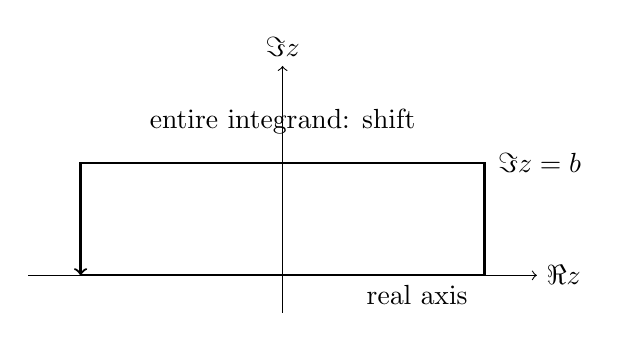
\begin{tikzpicture}[scale=0.95]
  \draw[->] (-3.4,0)--(3.4,0) node[right] {$\Re z$};
  \draw[->] (0,-0.5)--(0,2.8) node[above] {$\Im z$};
  \draw[thick,->] (-2.7,0)--(2.7,0)--(2.7,1.5)--(-2.7,1.5)--(-2.7,0);
  \node[right] at (2.75,1.5) {$\Im z=b$};
  \node[below] at (1.8,0) {real axis};
  \node at (0,2.05) {entire integrand: shift};
\end{tikzpicture}
\caption{Completing the square converts the oscillatory Gaussian to a vertically shifted Gaussian. Because the integrand is entire and decays on the vertical sides, Cauchy--Goursat shifts the real line to $\Im z=b$.}
\label{fig:cp-iv-0114-gaussian-shift-rectangle}
\end{figure}
